\section{Arquitetura do sistema}


\subsection{Solução}

No desenvolvimento desta solução, revela-se fundamental a organização do sistema em dois módulos distintos: um módulo responsável pela gestão da lógica de negócio, encarregada da execução das regras, validações e persistência de dados (\textit{Backend}); e um módulo de apresentação, dedicada à visualização e interação com a informação (\textit{Frontend}).

\subsection{Nível 1 - Contexto}

\subsubsection{Diagrama Lógico}

Na figura \ref{fig:diagram-lvl1-logical} encontra-se o diagrama lógico de nível. Este mostra os componentes desta arquitetura com um alto nível de abstração. Apenas é possível ver a exposição de 3 tipos de página \textit{web} para vários tipos de utilizadores: não registado, registado e administradores.   

\begin{figure}[h!tbp]
    \centering
    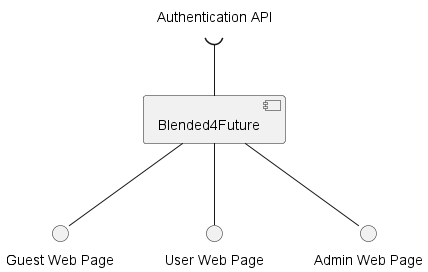
\includegraphics[width=0.5\linewidth]{capitulos/cap3-analisedoproblema/assets/arquiteturasistema/logical/logical_l1.png}
    \caption{Diagrama Lógico de Nível 1}
    \label{fig:diagram-lvl1-logical}
\end{figure}

\subsubsection{Diagrama Físico} 

A figura \ref{fig:diagram-lvl1-physical} demonstra o diagrama de físico de nível 1. Utiliza-se o \textit{port} 80 pois este é por norma utilizado em chamadas \Acrshort{HTTP} por este um protocolo baseado em \ACRshort{TCP}

\begin{figure}[h!tbp]
    \centering
    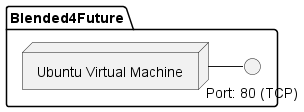
\includegraphics[width=0.5\linewidth]{capitulos/cap3-analisedoproblema/assets/arquiteturasistema/physical/physical_l1.png}
    \caption{Diagrama Físico de Nível 1}
    \label{fig:diagram-lvl1-physical}
\end{figure}





\subsection{Nível 2}

\subsubsection{Diagrama Lógico}

Na figura \ref{fig:diagram-lvl2-logical} é possivel ver um o anteriormente desmontrado na figura \ref{fig:diagram-lvl1-logical} com um menor nivel de abstração.
A este somam-se os conceitos de \textit{Frontend} e \textit{Backend}.

\begin{figure}[h!tbp]
    \centering
    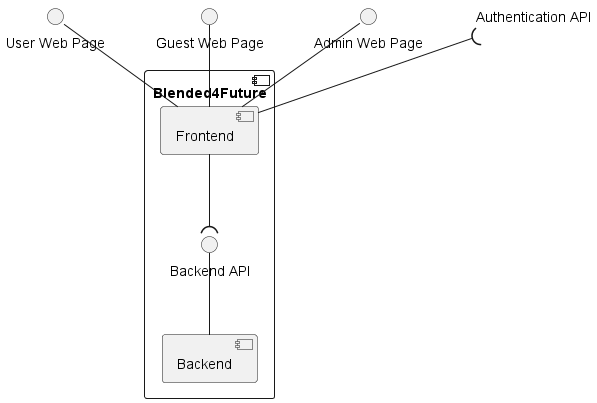
\includegraphics[width=0.7\linewidth]{capitulos/cap3-analisedoproblema/assets/arquiteturasistema/logical/logical_l2.png}
    \caption{Diagrama Lógico de Nível 2}
    \label{fig:diagram-lvl2-logical}
\end{figure}

\subsubsection{Diagrama Físico} 

A figura \ref{fig:diagram-lvl2-physical} demonstra o diagrama de físico de nível 2. Neste entende-se a função do servidor \gls{NGINX} como a de criação de duas rotas para \textit{Backend} e \textit{Frontend}, respetivamente \textit{'/api'} e \textit{'/'}.

\begin{figure}[h!tbp]
    \centering
    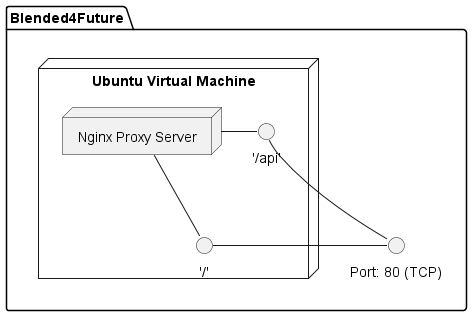
\includegraphics[width=0.6\linewidth]{capitulos/cap3-analisedoproblema/assets/arquiteturasistema/physical/physical_l2.png}
    \caption{Diagrama Físico de Nível 2}
    \label{fig:diagram-lvl2-physical}
\end{figure}




\subsection{Nível 3}

\subsubsection{Diagrama Lógico}

Com um nivel menor de abstração, a figura \ref{fig:diagram-lvl3-logical} apresenta aprofunda os modulos de \textit{Backend} e \textit{Frontend}. O primeiro é responsável pela logica de negócio e persistencia e, por tal, é detentor de uma aplicação Spring e de uma base de dados relacional \textit{MySQL}.

\begin{figure}[h!tbp]
    \centering
    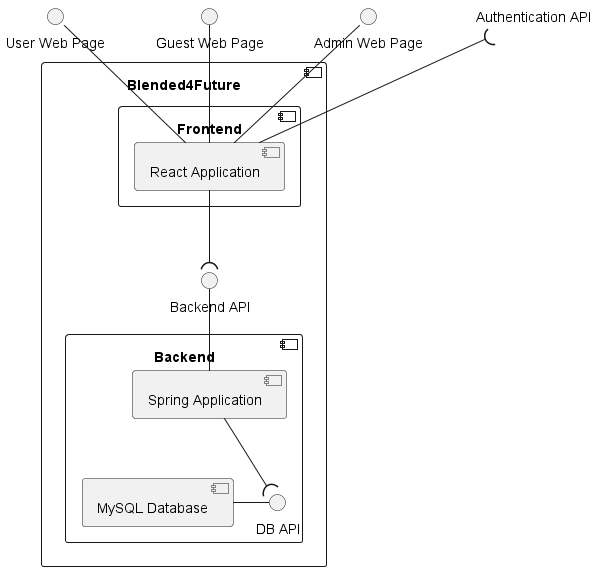
\includegraphics[width=0.8\linewidth]{capitulos/cap3-analisedoproblema/assets/arquiteturasistema/logical/logical_l3.png}
    \caption{Diagrama Lógico de Nível 3}
    \label{fig:diagram-lvl3-logical}
\end{figure}

\subsubsection{Diagrama Físico} 
A figura \ref{fig:diagram-lvl3-physical} demonstra o diagrama de físico de nível 3. Com este é possível verificar o mapeamento das duas rotas criadas pelo servidor \textit{proxy} \gls{NGINX} para os PORTS 3000 e 4000, escolhidos, pois são memoráveis. Foi feita ainda a escolha de encapsular as aplicações \textit{Backend} e \textit{Frontend} em imagens \gls{Docker} garantindo assim o seu funcionamento independentemente do \textit{hardware} escolhido.

\begin{figure}[h!tbp]
    \centering
    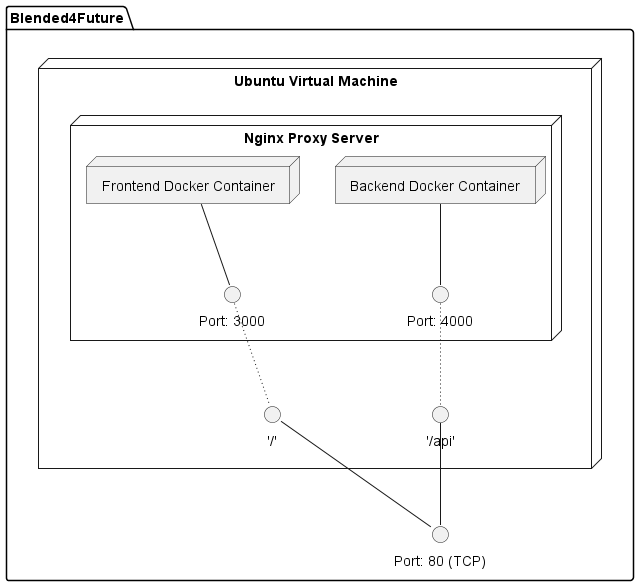
\includegraphics[width=0.7\linewidth]{capitulos/cap3-analisedoproblema/assets/arquiteturasistema/physical/physical_l3.png}
    \caption{Diagrama Físico de Nível 3}
    \label{fig:diagram-lvl3-physical}
\end{figure}





\subsection{Nível 4}

\subsubsection{Diagrama Físico} 

A figura \ref{fig:diagram-lvl4-physical} demonstra o diagrama de físico de nível 4. Dento das respetivas imagens \gls{Docker} é possível as aplicações  \textit{Backend} e \textit{Frontend} encapsuladas. No contexto do \gls{Docker} é necessário fazer um mapeamento dos \textit{ports} utilizados do ambiente interno (Imagem) para o externo (Máquina Virtual), por isso é possível ver o mapeamento dos ports, respetivamente, internos e externos, 8080 e 4000, no \textit{Backend} e 3000 e 3000 no \textit{Frontend}.

Em nota, é possível incluir a base de dados na imagem graças à funcionalidade \textit{Volumes} do Docker e esta pode persistir diretamente no \textit{hardware} da máquina virtual.

\begin{figure}[h!tbp]
    \centering
    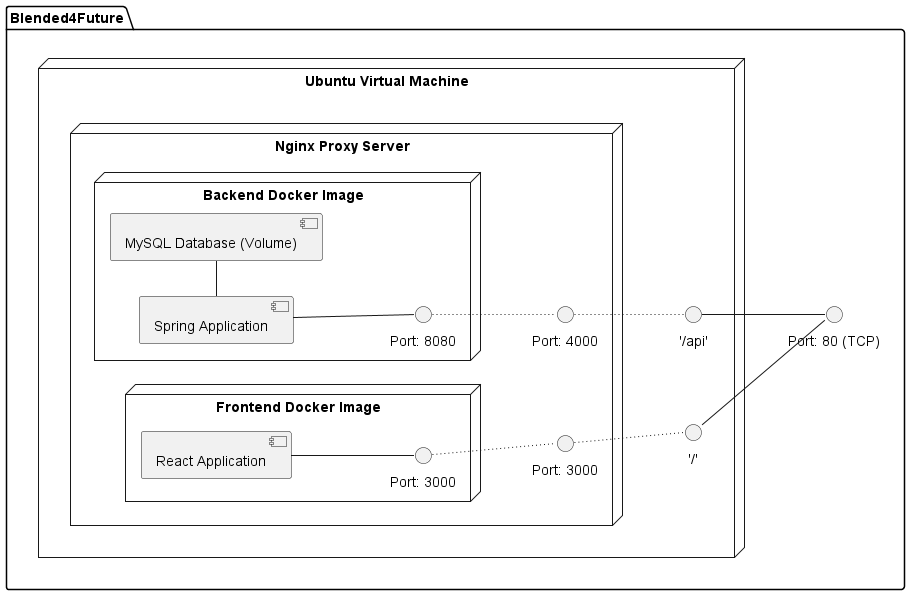
\includegraphics[width=\linewidth]{capitulos/cap3-analisedoproblema/assets/arquiteturasistema/physical/physical_l4.png}
    \caption{Diagrama Físico de Nível 4}
    \label{fig:diagram-lvl4-physical}
\end{figure}